% REV00 Tue 20 Jul 2021 08:12:01 WIB
% START Tue 20 Jul 2021 08:12:01 WIB

\chapter{Ketujuh}

% 11
\begin{figure}[htbp]
% h: here, where the figure appears in the text (use can always just use [h] )
% t: top,  top of the current page.
% b: bottom of the current page.
% p: page, top of the next available float space (sometimes end up being the end of the document).
\centerline{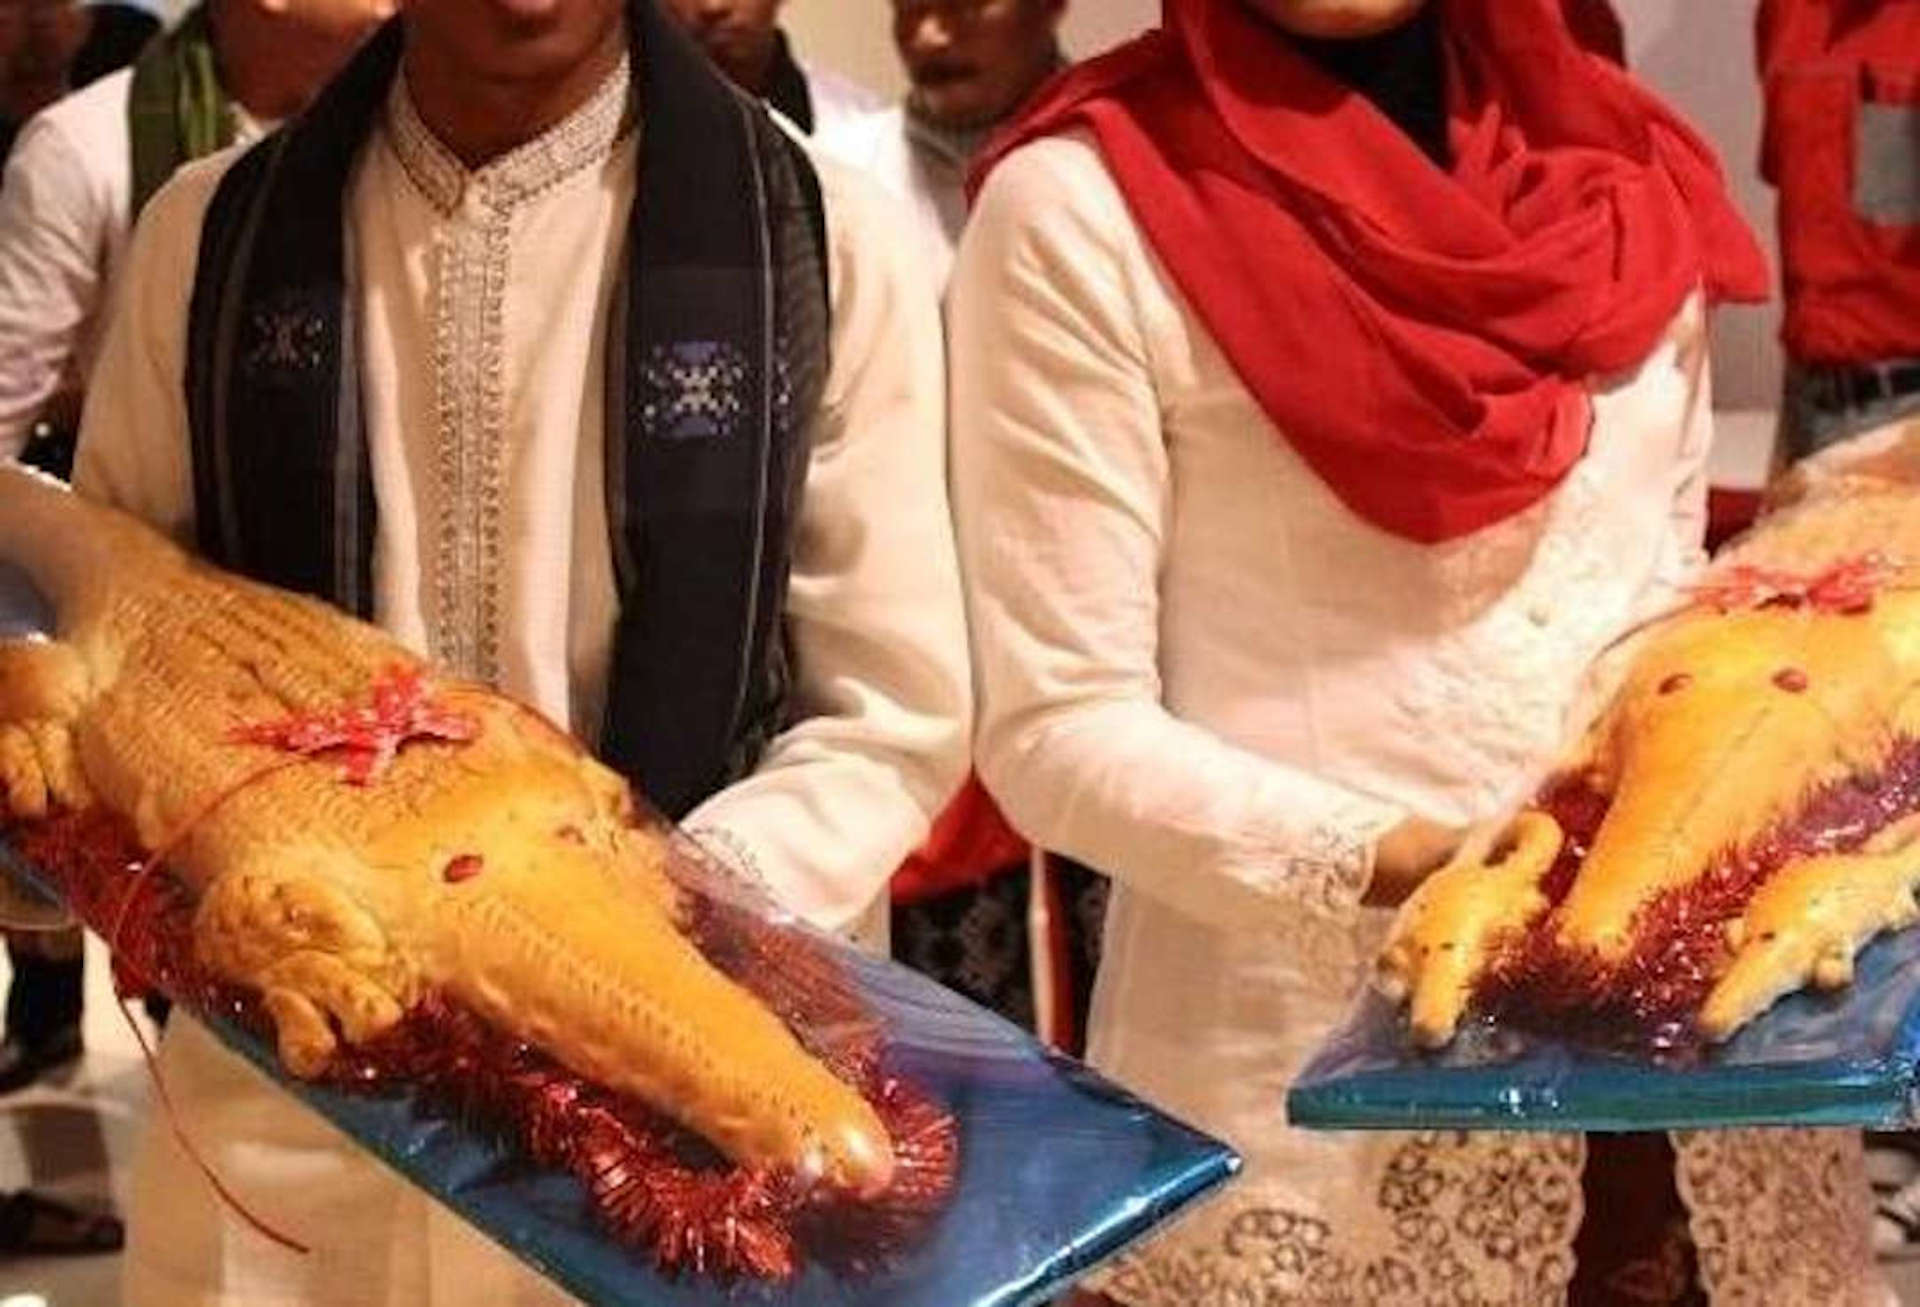
\includegraphics[scale=1.0]{01-07-01}}
\caption{“ROTI BUAYA yang harus selalu ada dalam pernikahan adat Betawi”. Sumber: Internet. Dalam budaya Betawi, dikatakan roti buaya adalah simbol buaya siluman yang dipercaya selalu ada dan menjadi pelindung di semua entuk atau sumber mata air (sumber kehidupan) di tanah Betawi. Lelaki harus memberikan sumber kehidupannya kepada perempuan.}
\label{01-07-01}
\end{figure}
%

Orang bilang, makna karaktermu adalah sifatmu. Dari hari ke hari, apa yang kamu pilih, apa yang kamu pikir dan apa yang kamu lakukan itulah yang akan menjadikanmu sebagai dirimu di masa depan. (Heraclitus)

Semester I berlalu, dan dia lulus di semua pelajaran dengan nilai-nilai yang lumayan. Semester II dia semakin berani, dan jarang ada di Kampus. Maklumlah di kampus kami saat itu hampir semua pelajaran tidak meminta absen. Kalau pun ada absen masih bisa titip teman, tanpa ada pemeriksaan.

“Mahasiswa itu orang dewasa yang harus berani bertanggung-jawab atas dirinya,” begitu kira-kira dosen kami dulu mengajarkannya. Padahal, malas lah mereka mengurus absen segala.

Duit dari BUMN sudah ditangan, dan dia pun mempertebal tabungan dengan ikut dagang kembang. Apa pasal? Itulah si Fitria, gadis manis mungil yang pandai melantunkan Qur’an. Semakin keluarga Fitria melarang-larang Satiri untuk menemuinya, semakin kuat tekad Satiri untuk segera menyuntingnya.

Anda tahu Hukum Ke-3 dari mas Newton: Ada aksi, maka ada reaksi dengan daya yang sama kerasnya ke arah yang berlawanan. Harus kumpulkan sejumlah uang!

Karena bukan anak tokoh, Satiri tidak pernah dianggap oleh ayahnya Fitria. Sekurang-kurangnya hingga saat itu. “Anak kuliah, apalah artinya anak kuliah, kalau calon besanku itu bukan siapa-siapa?”

Konon, babanya Fitria sudah berkali-kali berupaya menjodohkannya dengan beberapa ‘calon potensial’. Ada duda muda pengusaha tajir pemilik puluhan angkutan kota “si DOI”, Tanah Abang – Kebayoran Lama, jalur emas 24/7 pol. Ada juga anak pak Haji yang tanahnya super lebar di bilangan Kebon Jeruk!

Waktu mereka satu per satu didatangkan ke rumah, Fitria hanya diam saja mengkerut. Nyaris tidak mengatakan apa-apa. Setelah kepulangan mereka, babanya naik darah:

“Lu mau cari yang begimana lagi si?” (What the hell you want better than this, eh?! Be grateful!)

“A… aa… aye be… belon berani Ba?” katanya tambah mengerut. (I… I am… I am not dare enough yet, dad…)

“Awas, kalo elu macem-macem lagi ame calon yang ketiga besok ye?” ancam babanya. (Behave if you had to meet your next man I proposed for you!”)

Sementara itu, pertemuan kucing-kucingan antara keduanya terus berlanjut dibantu oleh adik-adik tersayang masing-masing pihak. Ada yang berjaga-jaga beberapa puluh meter dari rumah untuk memberi tanda jika baba Fitria tiba-tiba pulang saat malam-malam Satiri menggitarkan lagu-lagu cinta buat sang pujaan… (This part is true story, guys!)

Bagian yang kemudian, maaf ya sobat, saya tidak berani menceritakan rinciannya kepadamu. Tambah pula drama satu babak pro-kontra antara babanya Fitria dengan 'encing'nya (adik lelaki babanya Fitria) mengenai Satiri. Singkat cerita,

“Saya nikahkan engkau ananda Satiri bin Muhammad Zen dengan Fitria… dibayar tunai,” ijab babanya Fitria kepada Satiri, sambil buang muka. Duhhh…

“Saya terima nikahnya Fitria… dibayar tunai,” kabul Satiri dengan wajah sumringah penuh kemenangan.

Barang siapa yang memilih menerima tantangan, dia harus berani untuk menghadapi kekalahan ataupun kemenangan!

Orang sekampung mencintai mereka berdua sebagai pasangan cantik dan ganteng, pandai mengaji, dan baik hati. Dari tangan ke tangan mereka memindahkan ‘seserahan’ (marriage gifts) dari rumah Satiri ke rumah Fitria. Tidak kurang dari 300 meter jaraknya!

Ada kasur dan perlengkapannya serta ROTI BUAYA* (ini semua wajib buat pengantin Betawi), ada tas tangan dan pakaian buat pengantin wanita, handuk sepasang, ada sepatu dan sandal bagus dan lain-lainnya. Semuanya hasil jerih payah Satiri dagang kembang dan dari beasiswa Jenderal O. Semuanya mengalir penuh keceriaan, sambung menyambung tanpa hambatan…

Perjaka muda Satiri dan perawan muda Fitria sah menikah di awal Semester-2 Satiri di ITB. Lah, terus kuliahnya bagaimana?

Rupanya bukan cuma itu yang harus dihadapi Satiri. Babanya stress berat. Waktu pertama Satiri memberitahu babanya bahwa dia diterima untuk kuliah di ITB, babanya diam saja tidak tahu harus berkata apa atau bersikap bagaimana. Apa itu ITB mungkin dia juga kurang pasti.

“Iya terserah elu aja begimana nyari duitnya…”

Beberapa kari kemudian, tetangganya satu persatu menyalaminya, dan terus semakin banyak pula yang mendatanginya. Bahkan kenalan lama dari kampung sebelah juga datang, khusus untuk mengucapkan selamat kepadanya:

“Selamet ya Zen… Anak elu ini bakalan jadi insinyur, jadi orang kaya beneran. Bukan 'kaya gusuran'…”

('Kaya gusuran' adalah istilah untuk orang yang mendadak kaya karena menjual tanahnya ketika harga tanah melambung tinggi)

Di situlah babanya baru sadar bahwa anak sulungnya lagi bikin kantong emas yang bisa diandalkan. Tidak bakalan lama lagi dia hanya tinggal uncang-uncang kaki saja, tidak perlu lagi dagang kembang yang melelahkan. Anak gua bakal jadi insinyur, jadi insinyuur, jadi insinyuuur…

Nah, tiba-tiba di akhir semester-1 itu ia seperti disambar petir, dibangunkan dari mimpi indah: Anaknya memilih menikah…

“Abis dah abiiiis…” (this is the end, my love, the end…)

Babanya berkeluh menggumam seperti itu sepanjang hari, selama lebih dari seminggu, dan bahkan terus berkepanjangan. Di mata orang-orang tua jaman itu, ketika seorang anak menikah, maka putuslah sekolahnya. Berhentilah masa depannya. Habis…

Masih ada lagikah masalah lain yang harus dihadapi Satiri? Unfortunately, yes. Nasib belum mau berdamai kepadanya.

Sebagaimana layaknya pengantin baru, setelah ijab-kabul dan walimah pernikahannya Satiri tinggal di rumah mertua. Hari-hari pertama, hubungan antara Satiri dengan ayah mertuanya berjalan dingin, saling menghindari, menyapa seadanya.

Seminggu kemudian keadaan mulai memanas. Konfrontasi langsung tentu tidak mungkin ada. Manalah ada orang tua yang menginkan anak perempuannya segera menjadi janda. Satiri yang walaupun jenaka cukup sensitif membaui potensi percekcokan besar antara kedua mertuanya. Mungkin ini hanya ekses dari ‘kekalahannya’ menghadapi Satiri. Sebelum yang seperti itu terjadi, keputusan berat harus dibuat: Pindah ke rumah orang tua Satiri.

Fitria. Dari rumah gedongan, pindah ke rumah sederhana, untuk mengubahnya menjadi rumah cinta!

Menghadapi mertua, rasa sayangnya kepada Fitria yang luar biasa, dan menghadapi babanya sendiri secara bersamaan, semua itu adalah karena pilihan sadarnya.

Tentu saja Satiri kalang kabut, ketakutan. Sudah membuat istri kesayangannnya ikut menderita, dan membikin babanya tersiksa. Dia berupaya meyakinkan babanya bahwa dia tidak akan berhenti kuliah, dan tetap akan dapat uang beasiswa, dan juga tetap akan dagang kembang.

Berhasil? Tentu saja tidak, semua upayanya itu nyaris gagal total. Babanya semakin stress berat. “Ya Tuhan, aku sudah menjalankan sunahMu untuk menikah. Menghindari diri dari berzinah. Apa lagi yang harus aku lakukan?”
\\[10pt]


Sumber tulisan asli \url{https://www.facebook.com/reno.alamsyah.94/posts/10226542444573444}

